\documentclass[twoside]{article}

\usepackage{epsfig}
\usepackage{hyperref}
\usepackage{enumitem}

\setlength{\oddsidemargin}{0.0 in}
\setlength{\evensidemargin}{0.0 in}
\setlength{\topmargin}{-0.6 in}
\setlength{\textwidth}{6.5 in}
\setlength{\textheight}{8.5 in}
\setlength{\headsep}{0.75 in}
\setlength{\parindent}{0 in}
\setlength{\parskip}{0.1 in}

\title{Classification of Speech Acts in MOOC Forums}
\author{Kyle Shaffer \\ 
University of North Carolina at Chapel Hill \\
School of Information \& Library Science \\
shafferk@live.unc.edu}
\date{}

\begin{document}

\maketitle

\section{Introduction}\label{sec:introduction}
The increasing intersection of technology and education has greatly changed how both instructors and students view the delivery of courses. Today massive open online courses, or MOOCs, are the primary example of offering open course materials to anyone with an internet connection and the dedication and interest to complete the course. The ability to develop course content and offer remote access to these materials has indeed challenged the role of the in-person course offerings in ``brick and mortar'' institutions, and has allowed for an unparalleled number of students to learn from some of the most highly regarded instructors in the world at little to no cost. This has profound implications for equality in education, and is particularly salient given the steeply rising cost of college education within the United States. 
\par
However, this movement within online education is not without its challenges. Indeed, many have highlighted the extremely low completion rates compared with in-person course offerings and even the founder of Udacity, one of the largest current MOOC platforms, has publicly called the first iteration of their remote course offerings a ``lousy product.''\footnote{Slate Magazine, \url{http://www.slate.com/articles/life/education/2013/11/sebastian_thrun_and_udacity_distance_learning_is_unsuccessful_for_most_students.html}} The main message from these criticisms seems to be that the sheer volume of students who sign up and have access to these materials provides no indication for how successful students will be in completing the courses. The most severe conclusion to be drawn from this poor retention is that the goal of reaching these students isn't being met and perhaps investment in MOOCs should be greatly scaled back, or abandoned altogether. 
\par
Despite widespread disagreement about the effectiveness of MOOCs, there is little disagreement that many students are initially enrolling in these courses. The enrollment for any given course can quickly rise to thousands of students, and this presents a key challenge for instructors and other course managers in MOOCs. The problem, as stated above, is that few of these students complete these courses. With such large course enrollments, and the threat of many of these students dropping out, there is a unique opportunity to provide MOOC instructors with automated tools to alert them to student posts within discussion forums for greater effectiveness in intervention. That is, threads within these forums that contain many students posting about frustration or confusion with course materials could be flagged and brought to the attention of the instructor through an automated application that would classify posts and threads according to their need for intervention. 
\par
This present study aims to provide an experimental basis for developing such a tool by building predictive models and evaluating their performance in classifying discussion forum posts into speech act categories. Additionally, this study presents work on obtaining crowdsourced annotations from non-experts, and explores whether reliable annotations can be gathered using these methods for use in machine learning experiments. If these models are able to classify posts into different categories with an acceptable degree of accuracy, then this provides greater motivation for further developing software accessible by MOOC instructors that would alert her/him to posts within these forums that warrant instructor intervention. This would be far preferable to ignoring struggling students due to an inability to comb through and manually identify these posts. In addition to an assessment of the accuracy results, this study will also provide an analysis of the most useful features for use in these models by way of a feature ablation study. 
\par
The rest of the paper will proceed as follows. Previous work relevant to the present study is covered in the next section. In Section \ref{sec:data}, the speech act labels are defined and the dataset under analysis is presented. Following this, the method for collecting annotations from crowdsourced non-expert workers is presented as well as the supervised learning task and a description of the features used in the study. Finally, results and discussion are presented in Section \ref{sec:results} before concluding.

% RELATED WORK
\section{Related Work}
Two branches of previous work inform the present study. The first concerns computational approaches to the detection of speech acts within various application domains, while the second consists of a more varied set of analyses of student behavior within MOOCs. In what follows we provide context and previous work to help situate the present study.
\subsection{Speech Act Detection}
Computational methods of speech act detection have been applied to various domains with many different sets of speech acts to be detected. Early work in this area focused on detecting ``email speech acts'' specific to the message structure of email conversations \cite{cohen2004learning,carvalho2005collective}. These studies were some of the first to show the value of contextual evidence from an ongoing conversation in predicting the purpose of a single email, and this is directly applicable to the present study. Qadir and Riloff~\cite{qadir2011classifying} used support vector machines to evaluate the effectiveness of a variety of linguistic features in predicting sentence-level speech acts in veterinary medicine message board posts. Interestingly, the authors opted to use a more general set of four speech acts not tailored to the domain of analysis, but found domain-specific semantic features helpful when utilized in conjunction with n-grams and syntactical features.
\par
More closely related to the present work, Ravi and Kim~\cite{ravi2007profiling} trained linear classifiers using $n$-gram features to distinguish between six speech acts specific to a discussion forum dataset from an online course offered through the University of Southern California. The authors placed emphasis on detecting questions and answers in the forum and found classifiers to be most accurate in detecting questions. A follow-up to this study by Kim and Kang~\cite{kim2014towards} proposed a two-step classification approach in which domain-specific speech acts were identified and finally entire threads were classified as resolved or unresolved based on the sequence of speech acts within them. These studies inform our work here, however we instead investigate correlation between speech acts and student attrition as a motivation for attempting to predict them using independent binary classifiers.
% MOOC Behavior Analysis
\subsection{MOOC Student Behavior Analysis}
Much of the research concerning MOOCs has focused on student attrition rates and many of these works have employed predictive tasks to understand these phenomena. Chatruvedi~\emph{et al.}~\cite{chaturvedipredicting} focused on predicting instructor interventions. The authors combined thread-level features (e.g., number of posts, up-votes), aggregated post features (e.g., mean time-difference between posts), and last-post features (e.g., number of question words) to predict whether the next post will be written by an instructor. Ramesh~\emph{et al.}~\cite{ramesh2014uncovering} instead focused on constructing probabilistic models in which student engagement was modeled as a hidden layer to predict when instructors should intervene in order to retain students who become unmotivated throughout the duration of the course, and found these models to outperform those that utilize only observable variables. Additionally, Wen~\emph{et al.}~\cite{wen2014sentiment} used sentiment analysis to predict student drop-out. The authors found a significant correlation between the ratio of positive-to-negative sentiment words in forum posts and the number of student drop-outs on a particular week. 
\par
In addition to retention, other studies have investigated more general aspects of student engagement within MOOCs. Elouazizi~\cite{elouazizi2014point} focused on detecting point-of-view and cognitive engagement throughout MOOC discussion forums, finding that most of the linguistic behavior within these discussion forums suggests low cognitive engagement. Similarly, Wen~\emph{et al.}~\cite{wen2014linguistic} focused on predicting drop-out by considering the level of \emph{learner motivation} and \emph{cognitive engagement} reflected in student forum posts. Posts were classified into high/low motivation using a machine-learned classifier and into various levels of cognitive engagement using a list of abstract words. A survival analysis found that both level of motivation and cognitive engagement were negatively correlated with drop-out---students exhibiting higher motivation and cognitive engagement were more likely to complete the course. While these studies vary in their approaches and goals, they help to inform our work in integrating speech act detection with broader issues in student engagement and attrition within MOOCs.

% DESCRIPTION OF DATA
\section{Description of Dataset}\label{sec:data}
In the following sections, the dataset under analysis is described. First, the speech act definitions to be predicted are explained and defined, and then descriptive statistics on the MOOC dataset are presented along with some useful terminology on aspects of the MOOC.
% Speech act definition
\subsection{Speech Act Definitions}
The theory of speech acts arose out of literature in philosophy of language and sociolinguistics, and seeks to characterize sentences or utterances in terms of the purpose or function they serve within a broader discourse. An early authoritative taxonomy was provided by philosopher John Searle who defined several canonical examples of speech acts including \emph{directives} which compel the listener of an utterance to perform some action, and \emph{expressives} which serve to communicate the psychological or emotional state of the speaker. \cite{searle1976taxonomy} While these have been extremely useful in the fields of pragmatics and discourse analysis, computational approaches to speech act detection often employ speech act definitions specific to a domain of analysis as in Kim and Kang above. The present study follows this approach of defining speech acts specific to our domain of analysis.
\par
Seven speech acts were defined for annotation by crowdsourced workers.\footnote{The labeling process is explained in greater detail in section \ref{sec:crowdsource} below.} These speech acts describe several common purposes for writing posts within a MOOC and include \textbf{questions}, \textbf{answers}, \textbf{issues}, \textbf{issue resolutions}, \textbf{positive acknowledgement}, \textbf{negative acknowledgement}, and an \textbf{other} category. Examples of each category are provided in Table \ref{table:speech-acts} below. 
\par
\textbf{Questions} are defined as a request for information or clarification about course content, and may be posed in interrogative form or as a statement within the post. Common questions revolve around confusion with homework or quiz materials. \textbf{Answers} are defined as posts that contain an attempt to provide useful information in direct response to a question post, and it is noted that answers may not successfully fulfill a previously asked question, but must attempt to directly address a previously asked question. \textbf{Issues} can be viewed somewhat as an analogue to questions, except that issues are primarily in regards to course logistics as opposed to content to be learned. Common issues are directed at submitting homework assignments or other discrepancies about how material is delivered in the course, and it is important to note that issues are typically viewed in a negative light by instructors and may require their direct intervention. Likewise, \textbf{issue resolutions} are somewhat analogous to answers in that they (a) must be a direct response to a previously raised issue, and (b) function primarily to resolve an issue raised about the course. An important clue that may help identify issue resolutions is that instructors may be more likely to write them within a thread, however an issue resolution need not definitively resolve an issue. \textbf{Positive acknowledgment} and \textbf{negative acknowledgement} are speech act categories designed to capture sentiment-based posts throughout the forum, and express positive and negative sentiment respectively toward a previously written post. One difficult aspect of finding these speech acts is the requirement that they be written in direct response to a previous post, and this can contribute to confusion between the \textbf{negative acknowledgement} and \textbf{issue} categories. Finally, the \textbf{other} speech act serves as a category to capture all other speech acts that may be present within the threads. Given that MOOC students are free to write about whatever they choose, much of the writing is quite ``noisy'' with respect to the speech acts to be detected, and the \textbf{other} category serves as a label for these other categories which may range from general introductions to planning in-person study groups.
% MOOC Dataset
\subsection{MOOC Dataset}
The dataset under analysis is comprised of all published communication\footnote{The full dataset contains both published and deleted posts, and we are concerned here only with posts that were not deleted by an author.} within the discussion forums from a MOOC on Metadata\footnote{\url{https://www.coursera.org/course/metadata}} offered through the School of Information and Library Science at the University of North Carolina, Chapel Hill on the Coursera\footnote{\url{https://www.coursera.org}} platform. The course was taught over eight weeks from August to November of 2013, and had an initial enrollment of just over 27,000 students in its first week, with an ending enrollment of just under 26,000 in its final week, though not all of these students remained active throughout the duration of the MOOC. While the initial enrollments for the course are quite high, only 1,418\footnote{\url{http://jeffrey.pomerantz.name/2013/11/data-about-the-metadata-mooc-part-4/} } of the registered students completed enough course material to earn a statement of accomplishment. While this appears to be an extremely low completion rate, there are important caveats to consider about differences between the MOOC education environment and that of more traditional educational settings including marked differences in student motivation and reasons for enrollment~\cite{koller2013retention}.
\par
Throughout the duration of the MOOC, students were evaluated on eight weekly homework assignments that included short-answer and coding segments, and these along with a final exam made up the evaluation component of the course. Each of these homework assignments followed one of eight learning modules offered throughout the course, ranging from a broad theoretical introduction to metadata and organization schemas to specific domain applications including metadata for the web. The content of each learning module was presented through a set of video lectures recorded by the course instructor along with selected readings that were assigned each week. The instructor and one teaching assistant were responsible for managing the course and responding to students through the discussion forums.
\par
Before presenting summary statistics on the discussion forums, it is helpful to provide some terminology in order to clarify the unit of analysis for the present study. Students communicated with one another and with instructors of the MOOC through written messages or \textit{posts}, and these make up the most granular unit of analysis, and the main focus of our predictive task as outlined in section \ref{sec:prediction} below.\footnote{In truth, individual messages within the forums consisted of \textit{posts} which are top-level messages, and \textit{comments} which are structurally tied to a specific post and typically a response to it. We model these two messages types as different contextual features for our classifiers, but they will be referred to under the umbrella term \textit{posts} hereafter.} This statement/response structure of these messages makes speech act prediction particularly salient in this domain. A \textit{thread} is a collection of \textit{posts} and \textit{comments} that typically make up a distinct topic. Finally, a \textit{forum} is the coarsest unit of analysis, and is comprised of a collection of \textit{threads}. The discussion forums are comprised of these \textit{threads}, which themselves are comprised of individual \textit{posts}. Our dataset consists of 2,943 individual messages (2,166 \textit{posts} and 777 \textit{comments}), 425 threads, and 15 forums.

% SA examples table
\begin{table}[h]
\centering
{\footnotesize
\begin{tabular*} {0.7\textwidth} {r |p{6.3cm}}
Speech Act & Example\\\hline
Question & ``In Question 8 on the assignment I'm confused about the code formatting. In lectures, the instructor said syntax should be of the form X, but do you have to include Y? Any ideas what I'm doing wrong?'' \\ \hline
Answer & ``The answer here should follow the form of the practice problems. Hopefully that helps.'' \\ \hline
Issue & ``The wording for Question 6 was confusing and ambiguous. Please consider revising the wording or giving students the points for this question.'' \\ \hline
Issue Res. & ``We are aware of a glitch in our submission form for Homework 2. As a result, the last question has been awarded to each student as a free point.'' \\ \hline
Positive Ack. & ``I'm glad I'm not the only one stuck on this! That was definitely confusing me too!'' \\ \hline
Negative Ack. & ``The last question may have been difficult, but part of learning new material is working at it. No sense in complaining.'' \\ \hline
Other & ``Hi everyone!  I'm a web designer and extremely interested in this course!''
\end{tabular*}}
\caption{Speech Act Examples}
\vspace{-15pt}
\label{table:speech-acts}
\end{table}

% METHOD
\section{Method} \label{sec:method}
In this section the approach to the predictive task is presented. First, the method for obtaining crowdsourced human annotations is described, as well as steps taken to evaluate these annotations. Next, an explanation of the features generated and used by the classifiers in this study is presented. Finally, the classification method and algorithm used within the study are described. 
% Crowdsourcing
\subsection{Crowdsourced Data Collection} \label{sec:crowdsource}
In supervised machine learning, the goal is to train a model to identify a set of concepts based on representative features that are ``learned'' from a set of training data. More technically, supervised learning can be thought of as function approximation. That is, the assumption is that some as yet unknown function \textbf{\emph{f}} describes the relationship between a set of features \textbf{X} and a label \textbf{\emph{y}}, and the goal of supervised learning is to train a model to infer this function from a set of training data. This makes aspects such as feature engineering and selection extremely important, but also necessitates a set of good labels that supervised machine learning algorithms will use as their ground truth or ``gold standard'' to learn from. Often high-quality labels for the concepts to be predicted are not present or ready-made within the dataset, and this necessitates a first step of obtaining these labels.
\par
In the past, research studies have relied on experts to annotate datasets with gold-standard labels, but as the size of these datasets has grown this process has come more expensive, and in the most extreme cases is infeasible given the size of the dataset. However, in recent years crowdsourced options have become widely used among researchers as a way to obtain labeled datasets inexpensively and in a fraction of the time it would take for expert annotation. While there are concerns about the quality of the obtained labels, prior work has shown that aggregating redundant labels for each instance within a dataset can lead to improved quality as opposed to only collecting a single label per instance within the dataset \cite{sheng2008get}. Following this insight, labels for this study were collected using the crowdsourcing framework Amazon Mechanical Turk (hereafter MTurk).\footnote{\url{https://www.mturk.com/mturk/welcome}} MTurk allows for anyone with an internet connection to select Human Intelligence Tasks (HITs) posted by researchers, and complete simple tasks within HITs for a small compensation. 
\par
MTurk workers were first shown a set of speech act definitions as presented above, and also provided additional tips and examples to help them differentiate between speech acts that may be easily confused. Some of the posts within the dataset were easily identifiable as belonging to a particular speech act, and we provided MTurk workers with typical examples of these categories (see Table \ref{table:speech-acts} above). While we gave clear definitions of these speech acts, we found that these were not exhaustive, and therefore designated a final speech act, \textbf{other}, to serve as a placeholder for all posts that did not fit into any of the previous categories. This makes the \textbf{other} category extremely noisy, containing anything from introductions ("Hi everyone. I'm a web designer and extremely interested in this course!") to sharing tangential material ("sorry, this is not exactly relevant, but I could not stop myself from sharing..."), and this likely contributed to some confusion in the annotation process as detailed below. This \textbf{other} category, then, contains several speech acts that we left undefined since they were not relevant to the task of identifying meaningful student behavior within the MOOC. Often these speech acts were informal or conversational in nature, including introductions, organizing in-person study groups based on geographic location, and expressions of excitement about the course.
\par
To collect these annotations, we designed an interface presenting MTurk workers with an outlined post within a thread. MTurk workers were able to scroll throughout the thread and explore its context before labeling the outlined post with one or more speech acts ranging from none (by labeling the post as \textbf{other}) to all seven speech acts. Figure \ref{fig: interface} shows an example of this data collection interface. To help ensure worker quality and English-language proficiency we accepted annotations only from MTurk workers within the U.S. that had an acceptance rate of 95\% or greater. In addition we asked MTurk workers to provide justification for their answer as prior work has shown that users are more likely to submit high-quality work when asked to defend their answers. As a final set of precautions, we only allowed any given user to complete 30 annotations, and planted five "trap" annotation questions throughout the beginning of the HIT. These trap questions were thought to be trivially simple in the eyes of the authors, and we removed users who failed to answer three of these five correctly, assuming that failing these questions was the result of malicious or extremely careless work.

% Data collection interface figure
\begin{figure}[h]
\centering
\fbox{
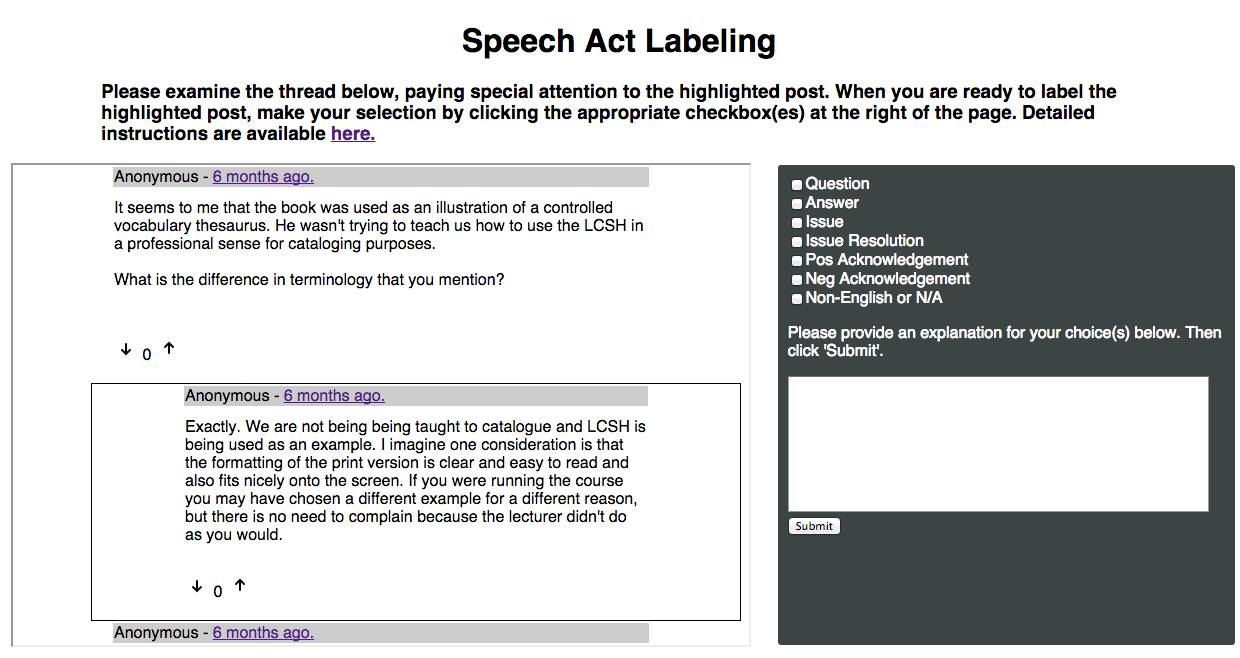
\includegraphics[width=0.8\textwidth]{imgs/turker_interface2} }
\caption{Example of MTurk interface for data collection.
\label{fig: interface} }
\end{figure}

\subsection{Evaluating Annotation Quality}
Using the above framework, five redundant annotations were collected for each post within the dataset. We then measured inter-annotator agreement with respect to each independent speech act using Fleiss' Kappa Agreement between the annotators. We also had an expert (one of the authors) annotate 30\% of the dataset and measured Cohen's Kappa Agreement between the expert annotations and the majority vote annotation from the MTurk workers, where the majority vote was taken to be the speech act that at least three annotators agreed upon for a given post. Cohen's Kappa Agreement scores between the MTurk workers and the expert annotator fell between 0.635 and 0.893, and these scores were found to be satisfactory given the obscurity of the annotation task, however it is acknowledged that agreement could be improved.
\par
Despite providing examples of each speech act and tips for how to differentiate between boundary cases, some speech acts were nonetheless still confusable. Given the informal writing in the majority of the threads, it is perhaps unsurprising that many of the posts were difficult to place cleanly into a speech act category with high agreement among MTurk workers. We attempted to identify speech act pairs that appeared naturally confusable and noticed that one speech act in particular, \textbf{positive acknowledgement}, appeared to frequently co-occur in annotations with several other speech acts, most notably \textbf{answer} and \textbf{other}. A qualitative look at some of these annotations made it clear why these categories may have been extremely difficult to distinguish between. For example, here is a post that received equal annotations for both \textbf{positive acknowledgement} and \textbf{other}: ``Hi I'm [name] from [location]. I'm currently working part-time as a cataloger, and part-time as a Digital Librarian. I've been a cataloger since 1990, but a digital librarian for only 2 months, so I"m [sic] here to learn all the things I've forgotten about metadata. Nice to meet you all.'' While the overall tone of this post is positive and friendly, it does not specifically convey positive sentiment or encouragement \emph{directly to a previous post}. Rather it serves as a general introduction and should have been labeled as \textbf{other}.

% Table for inter-annotator agreement
\begin{table}[h]
\centering
\begin{tabular*} {0.6\textwidth} { r | c | c }
\textbf{Speech Act} & \textbf{Fleiss' $\kappa$} & \textbf{Cohen's $\kappa$} \\ \hline
Question & 0.569 & 0.893 \\ \hline
Answer & 0.414 & 0.790 \\ \hline
Issue & 0.421 & 0.669 \\ \hline
Issue Resolution & 0.286 & 0.635 \\ \hline
Positive Acknowledgement & 0.423 & 0.768 \\ \hline
Negative Acknowledgement & 0.232 & 0.633 \\ \hline
Other & 0.337 & 0.625 \\
\end{tabular*}
\caption{Fleiss' and Cohen's Kappa statistics for inter-annotator agreement.}
\label{table: annotator-agreement}
\end{table}

Allowing MTurk workers to label posts into any number of speech act categories necessitated treating each speech act independently, and this has ramifications for the distribution of these labels throughout the dataset as shown in Table \ref{table:speech-act-distributions}. Readers should note that this independence assumption means that the reported percentages do not sum to 1, and this is a result of taking the majority vote of the MTurk worker annotations as the final speech act label for each post. Posts that had no majority vote (i.e. each speech act category received two or fewer annotations from MTurk workers) are not assigned a speech act, and instead are treated as a negative example for \emph{all} speech acts when building our independent binary classifiers.


% Table for speech act distributions
\begin{table}[h]
\centering
\begin{tabular*} {0.5\textwidth} { r | p{4cm} }
\textbf{Speech Act} & \textbf{\% of Dataset Labels} \\ \hline
Question & 12.6\\ \hline
Answer & 21.2 \\ \hline
Issue & 7.4 \\ \hline
Issue Resolution & 2.9 \\ \hline
Positive Acknowledgement & 34.9 \\ \hline
Negative Acknowledgement & 1.6 \\ \hline
Other & 9.5 \\
\end{tabular*}
\caption{Speech act distributions given majority vote annotations. Note that percentages do not sum to 1 due to independence between speech acts.}
\label{table:speech-act-distributions}
\end{table}

% Features
\subsection{Description of Features}\label{sec:features}
Beyond collecting gold-standard labels, perhaps the most important aspect of supervised learning is extracting and engineering quality features for the learning algorithm to use in the training stage. Various types of features were constructed for prediction of our speech act categories, and these are presented in the following section. 
\par
\textbf{LIWIC Features.} These features were constructed using the Linguistic Inquiry Word Count (LIWC) text analysis software.~\cite{tausczik2010psychological} LIWC features are designed to capture a variety of psychological aspects of written text, and these may be useful for predicting speech acts related to aspects of sentiment and cognitive engagement with course material in the forum. These are computed by comparing input text to various word list dictionaries correlated with different psychological and emotional states.
% LIWC features
\begin{itemize}[noitemsep,nolistsep]
\item{\textbf{Affect (8)} These features capture general positive and negative sentiment within posts, as well as more general emotions such as sadness anxiety, and the presence of emoticons.}
\item{\textbf{Cognitive Engagement (9)} These features attempt to measure more abstract aspects of posts including whether the post is comparing and contrasting items, expressing uncertainty, or considering a causal relationship.}
\item{\textbf{Personal Concern (9)} These features capture personal aspects of text within posts including personal accomplishments, money, and death.}
\item{\textbf{Linguistic (26)} Several more general linguistic aspects of the writing in posts were capture using these features, including relative and absolute word frequency counts, average word counts per sentence, counts for different verb tenses, as well as expressions such as quantification and negation.}
\item{\textbf{Perceptual (4)} These features attempt to capture aspects of text directly related to sense perception including hearing, feeling, and seeing.}
\item{\textbf{Social (4)} Features referencing social aspects such as other humans, family, or friends were computed with these features.}
\item{\textbf{Spoken (3)} Different features were computed to capture typically spoken linguistic features such as non-fluencies (``uh'', ``hmm'') and fillers (``blah'', ``you know'')}
\end{itemize}

\textbf{Manually constructed features.} In addition to the features computed using the LIWC software, several features were constructed from other aspects of thread posts.
% Manually constructed features
\begin{itemize}[noitemsep,nolistsep]
\item{\textbf{Sentiment features (4)} Sentiment features may be salient to particular speech acts, especially positive and negative acknowledgement. These features were computed by tabulating the number of percentage of positive and negative words that occurred in each post using wordlists constructed by Liu \emph{et al} (2005).~\cite{liu2005opinion}}
\item{\textbf{Unigram (100)} The terms present in a post may be predictive of the topic or content therein. To capture these more nuanced aspects of posts, the $\chi^2$ correlation was computed between each unigram and each target class independently. The top 100 terms per speech act category were then taken as features for each speech act category.}
\item{\textbf{Text Similarity (6)} Similarity between post types may be useful in training classifiers. Thus, cosine similarity metric was used to measure similarity between posts based on TF.IDF weighting scheme of terms in posts. Specifically, similarity between a post and the previous post; similarity with the first post in the thread; and the minimum, maximum, mean, and variance of the the similarity with the previous thread post were all computed as similarity features.}
\item{\textbf{Temporal Features (3)} Given that students were expected to complete homework assignments and quizzes, features were computed to measure the time in days, hours, and minutes between the time a post was written and the time the nearest homework assignment was due.}
\item{\textbf{Sequential Correlation (7)} Past work~\cite{carvalho2005collective} has shown that contextual and sequential features are helpful in predicting messages that occur in sequence. To exploit these features, the prediction confidence value of over all seven speech acts for the the previous post are used as features.}
\item{\textbf{Author (1)} The type of speech acts contributed in a discussion thread likely varies between instructors and students. To capture this, the author of a thread is represented in this binary feature where 1 indicates the post was written by an instructor and 0 indicates the post was written by a student.}
\item{\textbf{Link (1)} Link-sharing may be predictive of answers. We model link-sharing as a binary feature indicating the presence or absence of a hyperlink.}
\item{\textbf{Modal Verbs (2)} Model verbs were shown to be predictive in past work on discussion forum classification.~\cite{bhatia2012classifying} These features are captured by calculating the absolute and relative frequencies of common modal verbs in a post.}
\item{\textbf{Position (2)} The relative and absolute position of the post within the thread is given by this set of features.}
\item{\textbf{Post/Comment (1)} This binary feature indicates whether the post is a "top-level" post or a comment that is structurally tied to a previous post.}
\item{\textbf{Punctuation (13)} Punctuation features may be salient to several speech acts, but particularly to identifying questions. To capture this, relative and absolute frequencies of thirteen punctuation types were calculated for each post.}
\item{\textbf{Votes (1)} In addition to simply writing the posts, students can communicate with one another in the form of "voting" on posts. Students may "up-vote" a post they found particularly helpful or insightful, and conversely "down-vote" a post they found unhelpful or distracting. These vote tabulations were a part of the dataset and are utilized in the models for this study.}
\end{itemize}

% Prediction
\subsection{Predicting Speech Acts}\label{sec:prediction}
Given the labels described in Section \ref{sec:crowdsource} and the features as described in Section \ref{sec:features}, the predictive task is, again, to train classifiers using these features to classify posts into one of a set of seven speech act categories. In addition, this task was formulated as a binary classification problem in which seven classifiers (one per speech act) were each trained and tested independently to detect one particular speech act. Formulating the experiments as binary classification tasks in which a classifier need only predict whether the speech act of interest is present or absent in each instance within the dataset has the advantage of  simplifying this problem, and this may give these predictive models a better chance at obtaining high performance.
\par
Several popular models are available for binary classification. Logistic Regression was chosen as the model for performing this classification task, and in particular a Python implementation\footnote{\url{http://scikit-learn.org/stable/modules/generated/sklearn.linear_model.LogisticRegression.html}} was used to build the models using the Scikit-Learn machine learning library.\footnote{\url{http://scikit-learn.org/stable/}} Logistic Regression is modeled by the following linear equation $Y=b_0+\sum{(b_i X_i)}+\epsilon$ where $Y$ = $\left\{ {0,1} \right\}$ is the categorical dependent variable (presence or absence of a speech act) to be predicted. This is the same basic representation as Linear Regression, however in Logistic Regression, $Y$ is rather the probability of a predicted binary outcome instead of a real-valued output as in Linear Regression. However, both models have the advantage of a straightforward interpretation of modeling the outcome variable, or label, as the result of some linear combination of a set of independent variables, or features.
\par
Models were trained and tested using 10-fold cross validation and evaluated in terms of mean average precision on held-out test sets across these 10 folds. Additionally, an ablation analysis was run to determine which features were most informative for the models in this study, and these results are presented in Section \ref{sec:results} below. Evaluating model performance in terms of average precision has several advantages over other popular metrics such as precision or recall which are often used in classification tasks. While these latter metrics are informative for displaying a snapshot of the performance of a classifier, they leave an incomplete picture of performance on average, and do not directly address the tradeoffs inherent between precision and recall in any classification task. Average precision provides a more nuanced picture of model performance by displaying how precision varies \emph{as a function of recall}, instead of simply presenting these metrics side-by-side. While, average precision may be less straightforward to interpret, it can be thought of graphically as the area under a two-dimensional precision-recall curve where the x-axis depicts increasing levels of recall, and the y-axis depicts increasing levels of precision. A curve whose area is summed to 1 would then denote a model that achieves perfect precision at every stage of recall, or an average precision score of 1. Finally, Logistic Regression uses a \emph{C} parameter that controls regularization of the model given a misclassification cost on the training set. This parameter was tuned by performing 5-fold cross-validation on each training set of the 10 training-test set pairs, and using an exhaustive grid search algorithm to tune \emph{C} across the values $2^x$, where \emph{x} = -5, -4, -3, -2, -1, and 0. 

% RESULTS AND DISCUSSION
\section{Results and Discussion} \label{sec:results}
In this section, results of the classification task are presented with particular focus on results from a feature ablation analysis investigating the impact made by different groups of features. Table \ref{tab:results} shows the results of the analysis, with scores marked in bold for features that made the greatest positive contribution for each speech act. The first row depicts the results for classifiers built with all features constructed from the forum data. Subsequent rows show performance of classifiers built without the indicated set of features to evaluate their contribution to the predictive task. Therefore, a decrease in performance in any of these rows indicates a positive predictive contribution from this feature group.\footnote{Note that statistical significance is not reported for the ablation analysis, and readers should take this caveat into account when interpreting results.} All scores are in terms of average precision (AP).
\par
Overall, performance seems to be somewhat dictated by the proportion of the dataset that contains each speech act category. That is, if we look over the AP scores in Table \ref{tab:results}, we see that performance is roughly proportionate to the percentage of labels throughout the dataset as reported in Table \ref{table:speech-act-distributions}. This makes intuitive sense given that the more examples a classifier has to learn from, the better chance it will likely have of identifying this concept in a previously unseen test set. In addition, it is encouraging to see the two of the highest scores occur in the \textbf{question} and \textbf{answer} categories as this conforms to prior research results, and these are likely speech acts that would be of primary concern to a MOOC instructor.
\par
Beyond these observations, several more nuanced results are worth noting. First, and perhaps most striking, is the performance of the \textbf{negative acknowledgment} classifier. The performance over all features is substantially lower than all other speech act classifiers (25.3\% AP), but given the sparsity of this speech act within the dataset (1.6\%) these results are quite surprising. This is doubly encouraging since this speech act is likely of high priority for instructor intervention, and these results suggest that posts with negative sentiment can be identified even if they are very sparse throughout the forum. Interestingly, however, the ablation analysis results show that sentiment features are not most salient for predicting this category, and this may be the result of more subtle expressions of negative sentiment throughout the forums.
\par
Other results from the ablation analysis seem to conform to prior intuition about informative features for particular speech acts. For instance, it is encouraging to see that the punctuation features are most informative for questions, given that punctuation such as question marks are likely easy signals for classifiers to identify within the data in order to effectively predict the presence of questions within these forums. Likewise, the author feature which indicates whether a post was written by a student or instructor stands out as the most predictive feature for identifying issue resolutions, and this conforms with the notion that instructors are more likely to write posts attempting to resolve issues than students. Finally, unigram features are helpful in predicting many of the speech act categories, and are the most predictive feature group for four out of the seven speech acts. This suggests that topical or semantic information communicated by the words particular to each speech act are useful in identifying these categories, and this makes sense. However, this comes with a caveat that while unigram features are helpful in this classification task, it is highly unlikely that \emph{the same} unigrams would be informative over different types of MOOCs, and these features would likely need to be computed for individual MOOC to replicate the results found here.
\par
While these results indicate progress being made in this classification task, some puzzles remain. For instance, in addition to punctuation, social features are tied for most informative in predicting questions, and it is not immediately clear why this would be the case. That is, questions do not on their face appear more likely to draw discussion of social issues than any of the other speech acts, but this may necessitate further investigation. Conversely, affective features seemed to be good candidates for predicting several speech acts including positive and negative acknowledgement as well as issues, however these features make no substantial contribution to \emph{any} speech act and actually increase performance upon their removal for questions, issue resolutions, and other. This may be the result of this feature overlapping somewhat with the sentiment feature group, however removal of this feature group had little positive or negative effect on performance.

% Ablation Study Results
\begin{table}[t]
  \centering
  {\footnotesize
    \begin{tabular*}{\textwidth}{rcccccccc}
          & \multicolumn{1}{c}{question} & \multicolumn{1}{c}{answer} & \multicolumn{1}{c}{issue} & \multicolumn{1}{c}{issue resolution} & \multicolumn{1}{c}{positive ack.} & \multicolumn{1}{c}{negative ack.} & \multicolumn{1}{c}{other} \\ \hline
    all features  & \multicolumn{1}{c}{0.709} & \multicolumn{1}{c}{0.673} & \multicolumn{1}{c}{0.604} & \multicolumn{1}{c}{0.489} & \multicolumn{1}{c}{0.756} & \multicolumn{1}{c}{0.253} & \multicolumn{1}{c}{0.609} \\\hline
    -affective & 0.713 & 0.670 & 0.600 & 0.514 & 0.755 & 0.251 & 0.620  \\
    -author & 0.706 & 0.674 & 0.604 &  \textbf{0.451} & 0.754 &  0.252 & 0.612 \\
    -cognitive & 0.724 & 0.682 & 0.594 & 0.485 & 0.758 & 0.263 & 0.614  \\
    -context & 0.709 & 0.638 & 0.600 & 0.467 & 0.751 & 0.291 & 0.600 \\
    -cosine & 0.711 & 0.672 & 0.604 & 0.506 & 0.757 & 0.239 & 0.611  \\
    -linguistic & 0.707 & 0.668 & 0.580 & 0.509 & 0.752 & 0.270 & 0.604 \\
    -links & 0.707 & 0.672 & 0.605 & 0.489 & 0.757 & 0.251 & 0.612  \\
    -modal & 0.707 & 0.673 & 0.604 & 0.491 & 0.756 & 0.251 & 0.614 \\
    -perceptual & 0.712 & 0.674 & 0.598 & 0.488 & 0.762 & 0.252 & 0.611 \\
    -personal\_concerns & 0.707 & 0.602 & 0.486 & 0.550 & 0.757 & 0.252 & 0.616  \\
    -temporal & 0.706 & 0.605 & 0.605 &  0.489 & 0.761 & 0.290 & 0.614  \\    
    -position & 0.710 & 0.604 & 0.598 & 0.488 & 0.758 & 0.249 & 0.614 \\
    -post\_comment & 0.710 & 0.609 & 0.672 & 0.503 & 0.756 & \textbf{0.228} & 0.617 \\
    -punctuation &  \textbf{0.581} & 0.604 & 0.661 & 0.482 & 0.751  & 0.249 & 0.608 \\
    -sentiment & 0.707 & 0.604 & 0.604 & 0.498 & 0.758 & 0.242  & 0.614 \\
    -social & \textbf{0.581} & 0.604 & 0.604 & 0.482 & 0.751 & 0.249 & 0.608 \\
    -spoken & 0.707 & 0.605 & 0.594 & 0.491 & 0.760 & 0.253 & 0.614  \\
    -unigram & 0.666 & \textbf{0.547} & \textbf{0.553} &  0.505 & \textbf{0.714} &  0.257 & \textbf{0.587}  \\
    -votes & 0.724 & 0.604 & 0.663 & 0.504 & 0.751 & 0.251 & 0.607 \\\hline
\end{tabular*} }
  \caption{Feature Ablation Study Results.}    
  \vspace{-15pt}  
  \label{tab:results}
\end{table}

% CONCLUSION
\section{Conclusion}\label{sec:conclusion}
This study sought to evaluate the performance of binary classifiers on predicting seven speech act categories specific to posts within a MOOC forum. The study also investigated the feasibility of obtaining high-quality gold-standard labels for the machine learning task using crowdsourced annotations from non-experts. This latter contribution is especially insightful given the obscurity of the definitions of labels we attempted to collect. Results from inter-annotator agreement within this study show that aggregating multiple annotations per instance within a dataset greatly improves the quality of the annotations over collecting only a single annotation per instance. This may help encourage researchers to use services such as Mechanical Turk to collect data from more complex labeling tasks than have been previously explored, however important caveats were also presented regarding difficulties in defining these somewhat obscure labels for MTurk workers. 
\par
In addition, the feature ablation study led to several insights about the usefulness of different types of features for predicting the presence of each speech act in a given thread. Unigram features were helpful for many of the speech acts, but not all in this analysis. Additionally, several features were helpful only in predicting particular speech acts such as punctuation for questions and post author features for issue resolution. Surprisingly, several features that seemed \emph{a priori} predictive of speech acts (cognitive processes and cosine similarity features) were not as helpful in the analysis as previously thought.
\par
There is ample room for future work and improvements in the area of speech act predictions. Regarding annotation collection from non-expert MTurk workers, exploring the effectiveness of different types of definitions on subsets of the data could be useful in homing in on the most effective method for describing these somewhat obscure categories. Great care was taken in this study to make the speech act definitions as clear as possible, but improvements could be made in helping annotators differentiate between closely related speech acts. In terms of improving classifier performance, perhaps using 20-  or 50-fold cross validation would help performance by using larger training sets for the models to learn from. The results also suggest that the words actually written in the posts are among the most informative for our classifiers, and thus perhaps exploring the use of bigrams in addition to unigrams could be of help. In addition, it is not clear how well these results generalize to other MOOCs in different disciplines. That is, it is highly likely that writing is quite different from course to course, and great care may need to be taken in developing classifiers for MOOCs in different disciplines. For instance, it is highly unlikely that the unigrams used in the present study would be the best choice unigrams for an analysis run a different MOOC. However, given the difficulties and challenges in collecting gold-standard labels and training and testing classifiers on this crowdsourced data, the results obtained are encouraging and speak to great potential for future work in this area.

\bibliographystyle{unsrt}
\bibliography{root.bib}

\end{document}

